\hypertarget{_s_c_p_i__specific_cmds_8h}{\section{scpi/\-S\-C\-P\-I\-\_\-specific\-Cmds.h File Reference}
\label{_s_c_p_i__specific_cmds_8h}\index{scpi/\-S\-C\-P\-I\-\_\-specific\-Cmds.\-h@{scpi/\-S\-C\-P\-I\-\_\-specific\-Cmds.\-h}}
}
This graph shows which files directly or indirectly include this file\-:\nopagebreak
\begin{figure}[H]
\begin{center}
\leavevmode
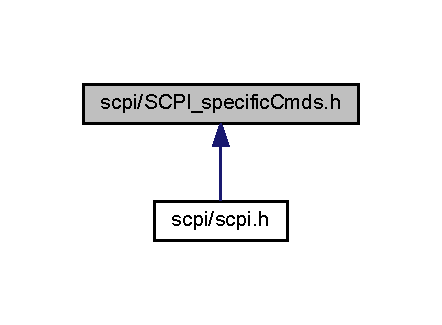
\includegraphics[width=212pt]{_s_c_p_i__specific_cmds_8h__dep__incl}
\end{center}
\end{figure}


\subsection{Detailed Description}
This file includes the functions for registering the application specific commands and the related callback functions

These commands and their associated callback functions can be edited to suit the application in use, though they should follow the guidelines and conventions laid out in I\-E\-E\-E 488.\-2-\/1992 and S\-C\-P\-I-\/1999

Please follow the information in the parser documentation and the file S\-C\-P\-I\-\_\-specific\-Cmds.\-c on how to add or change message headers, commands and parameters

To register a new command device specific tree node, add a register\-Child() call to the function register\-Specific\-Commands() with the form \char`\"{}err += register\-Child(\-C\-H\-I\-L\-D\-\_\-\-L\-O\-N\-G\-\_\-\-N\-A\-M\-E, P\-A\-R\-E\-N\-T\-\_\-\-S\-H\-O\-R\-T\-\_\-\-N\-A\-M\-E,
\-B\-O\-O\-L\-\_\-\-I\-S\-\_\-\-H\-E\-A\-D\-E\-R\-\_\-\-O\-N\-L\-Y, B\-O\-O\-L\-\_\-\-I\-S\-\_\-\-Q\-U\-E\-R\-Y, C\-A\-L\-L\-B\-A\-C\-K\-\_\-\-H\-A\-N\-D\-L\-E);\char`\"{}, where\-:


\begin{DoxyItemize}
\item C\-H\-I\-L\-D\-\_\-\-L\-O\-N\-G\-\_\-\-N\-A\-M\-E is the long form of the name of the child node to be registered.
\end{DoxyItemize}


\begin{DoxyItemize}
\item P\-A\-R\-E\-N\-T\-\_\-\-S\-H\-O\-R\-T\-\_\-\-N\-A\-M\-E is the short form of the name of the parent of the child node to be registered. This must be an already existing node.
\end{DoxyItemize}


\begin{DoxyItemize}
\item B\-O\-O\-L\-\_\-\-I\-S\-\_\-\-H\-E\-A\-D\-E\-R\-\_\-\-O\-N\-L\-Y is a boolean value that indicates if the node being registered is a header only (i.\-e. is not a command) or not.
\end{DoxyItemize}


\begin{DoxyItemize}
\item B\-O\-O\-L\-\_\-\-I\-S\-\_\-\-Q\-U\-E\-R\-Y is a boolean value that indicates if the node being registered my be queried or not.
\end{DoxyItemize}


\begin{DoxyItemize}
\item C\-A\-L\-L\-B\-A\-C\-K\-\_\-\-H\-A\-N\-D\-L\-E is a pointer to the function to be associated with this child if it is a command, or N\-U\-L\-L if it is a header only.
\end{DoxyItemize}

For further information on the operation of register\-Child() please see the function description.

All string literals M\-U\-S\-T be in upper case and enclosed in quotation marks.

Node long and short names must conform to the standard as outlined by S\-C\-P\-I-\/99 in 6.\-2.\-1

All tree nodes are children of at least \char`\"{}\-R\-O\-O\-T\char`\"{}. Changes to the number of node registered should be reflected by the user in the number defined for T\-R\-E\-E\-\_\-\-C\-H\-I\-L\-D\-\_\-\-L\-I\-M\-I\-T in \hyperlink{scpi_8h}{scpi.\-h} 